%----------------------------------------------------------------------------------------
% Contenido del Informe - Resultados
%----------------------------------------------------------------------------------------
\section{Resultados}

A continuación, se presentan los resultados obtenidos a partir de la implementación del ajuste exponencial por mínimos cuadrados y de los cálculos solicitados en cada uno de los puntos del trabajo práctico. Los valores fueron obtenidos utilizando el notebook de Google Colab desarrollado para este proyecto.

\subsection{Ajuste exponencial de los datos}

Aplicando el método de mínimos cuadrados sobre los datos experimentales se obtuvo el siguiente modelo exponencial:

\[
Q(t)=274.573649\,e^{-0.000684635\,t}
\]

donde:

\begin{itemize}
    \item $A=274.573649$
    \item $B=-0.000684635$
    \item Error Cuadrático Medio (ECM): $76.807906$
\end{itemize}

En la Figura \ref{fig:ajuste} puede observarse el ajuste obtenido entre los datos experimentales y la curva exponencial.

\begin{figure}[H]
\centering
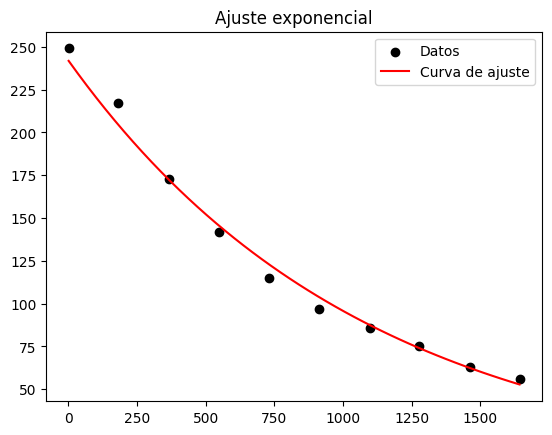
\includegraphics[width=0.82\textwidth]{imagenes/ajuste_exponencial.png}
\caption{Ajuste exponencial obtenido mediante mínimos cuadrados.}
\label{fig:ajuste}
\end{figure}

\subsection{Punto 1: Fecha estimada de cierre}

Utilizando el modelo obtenido se determinó el instante en el cual la producción diaria alcanza el valor de cierre establecido.

Se obtuvo un tiempo de:

\[
t=6176\ \text{días}
\]

Tomando como fecha inicial el 1 de enero de 2018, la fecha estimada de cierre corresponde al:

\[
\boxed{\text{28 de noviembre de 2034}}
\]

\subsection{Punto 2: Producción acumulada}

A partir de la integración del modelo exponencial se calcularon los volúmenes de producción acumulada.

Los resultados obtenidos fueron:

\begin{itemize}
    \item Producción total estimada: \textbf{394930.73 m$^3$}
    \item Producción extraída: \textbf{270555.65 m$^3$}
    \item Producción remanente: \textbf{124375.08 m$^3$}
\end{itemize}

Esto representa:

\begin{itemize}
    \item Producción extraída: \textbf{68.51\%}
    \item Producción remanente: \textbf{31.49\%}
\end{itemize}

La Figura \ref{fig:torta} muestra la distribución porcentual entre la producción extraída y la producción remanente.

\begin{figure}[H]
\centering
% If the image file is missing, show a framed placeholder instead of failing
\IfFileExists{imagenes/produccion_acumulada.png}{%
    \includegraphics[width=0.55\textwidth]{imagenes/produccion_acumulada.png}%
}{%
    \fbox{\parbox[b][0.28\textheight][c]{0.55\textwidth}{\centering Imagen ``produccion_acumulada.png'' no disponible.}}%
}
\caption{Distribución de la producción acumulada.}
\label{fig:torta}
\end{figure}

\subsection{Punto 3: Producción acumulada del 50\%}

Se determinó el instante en el cual la producción acumulada alcanza el 50\% de la producción total estimada.

Los resultados obtenidos fueron:

\begin{itemize}
    \item Producción acumulada correspondiente al 50\%: \textbf{197465.37 m$^3$}
    \item Tiempo: \textbf{992.28 días}
    \item Fecha: \textbf{18 de septiembre de 2020}
\end{itemize}

\subsection{Punto 4: Valor económico de la producción remanente}

El notebook calcula el valor económico de la producción remanente considerando:

\begin{itemize}
    \item Conversión de m$^3$ a barriles mediante el factor 6.28981.
    \item Precio del petróleo de \textbf{US\$62 por barril}.
\end{itemize}

Con estos datos se obtuvo el valor económico de la producción remanente desde el 2 de julio de 2022 hasta la fecha estimada de cierre.

\subsection{Punto 5: Producción anual}

Finalmente, se calculó el valor económico anual de la producción desde el año 2022 hasta el cierre del yacimiento.

La Figura \ref{fig:barras} presenta la evolución anual obtenida.

\begin{figure}[H]
\centering
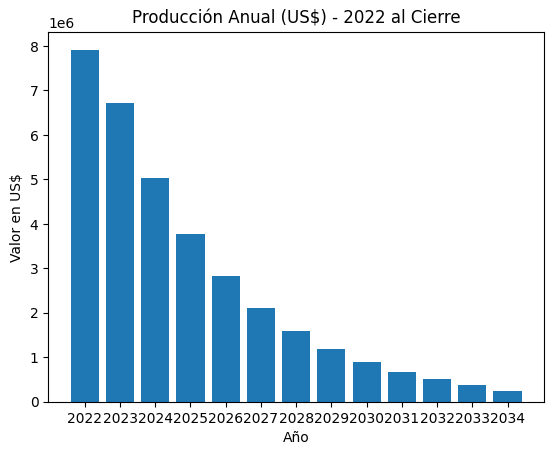
\includegraphics[width=\textwidth]{imagenes/produccion_anual.png}
\caption{Valor anual de la producción desde 2022 hasta la fecha estimada de cierre.}
\label{fig:barras}
\end{figure}

Como puede observarse, el valor económico anual disminuye progresivamente con el paso de los años, comportamiento consistente con el modelo exponencial ajustado para la producción del yacimiento.